% This chapter should describe what was actually produced: the programs which were written, the hardware which was built or the theory which was developed. Any design strategies that looked ahead to the testing stage should be described in order to demonstrate a professional approach was taken.

% Descriptions of programs may include fragments of high-level code but large chunks of code are usually best left to appendices or omitted altogether. Analogous advice applies to circuit diagrams or detailed steps in a machine-checked proof.

% The implementation chapter should include a section labelled "Repository Overview". The repository overview should be around one page in length and should describe the high-level structure of the source code found in your source code repository. It should describe whether the code was written from scratch or if it built on an existing project or tutorial. Making effective use of powerful tools and pre-existing code is often laudable, and will count to your credit if properly reported. Nevertheless, as in the rest of the dissertation, it is essential to draw attention to the parts of the work which are not your own. 

% It should not be necessary to give a day-by-day account of the progress of the work but major milestones may sometimes be highlighted with advantage.

% practical contributions.
% present deadlocks \& performance tests.
% reusable modules.

% Live testing revealed many subtle bugs, deadlocks, and performance issues (memory usage, messages dropped due to bugs preventing leaders from always advancing) that were time consuming to debug. However they helped me to flesh out a pacemaker algorithm based on these ad-hoc fixes that we have proven both correctness and liveness for. I also improved the ease of implementability based on practicalities I discovered during implementation (eg. using node offset and hashes to compare nodes)

% --- directory forest stuff
\definecolor{foldercolor}{RGB}{124,166,198}

\tikzset{pics/folder/.style={code={%
	\node[inner sep=0pt, minimum size=#1](-foldericon){};
	\node[folder style, inner sep=0pt, minimum width=0.3*#1, minimum height=0.6*#1, above right, xshift=0.05*#1] at (-foldericon.west){};
	\node[folder style, inner sep=0pt, minimum size=#1] at (-foldericon.center){};}
	},
	pics/folder/.default={20pt},
	folder style/.style={draw=foldercolor!80!black,top color=foldercolor!40,bottom color=foldercolor}
}

\forestset{is file/.style={edge path'/.expanded={%
		([xshift=\forestregister{folder indent}]!u.parent anchor) |- (.child anchor)},
		inner sep=1pt},
	this folder size/.style={edge path'/.expanded={%
		([xshift=\forestregister{folder indent}]!u.parent anchor) |- (.child anchor) pic[solid]{folder=#1}}, inner ysep=0.6*#1},
	folder tree indent/.style={before computing xy={l=#1}},
	folder icons/.style={folder, this folder size=#1, folder tree indent=3*#1},
	folder icons/.default={12pt},
}
% ---
\textit{In this chapter we describe the architecture of our implementation [\ref{overview}], present a specification and proof of correctness and liveness for our pacemaker [\ref{spec}], describe key optimisations implemented [\ref{performance}], present our load generator and experiment scripts which will be used in evaluation [\ref{benchcode}], and give an overview of the repository structure [\ref{repo}].}

\section{Architectural overview} \label{overview}

\begin{figure}[h!]
\centering
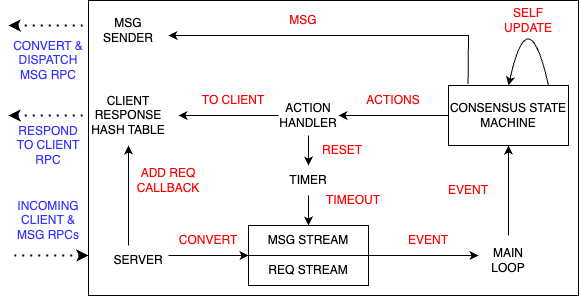
\includegraphics[scale=0.6]{nodediagram.png}
\caption{Architecture of a node.}
\label{nodediagram}
\end{figure}

The core implementation of the HotStuff algorithm (section \ref{spec}) is implemented in the \textit{consensus} module. The main function provided by this module is \textit{advance}, which delivers some event (such as an incoming message, client request or timeout) to the consensus state machine and returns an updated state and a list of actions (such as sending a message to another node or responding to a client request) to be carried out. This architecture is inspired by the \href{https://github.com/Cjen1/OCons}{OCons }project\footnote{At the time I began implementation the OCons project was still under development, so I was unable to use the code in my project.}, which was developed by my project supervisor. The \textit{consensus} module contains both a chained and unchained implementation that share a common signature, so can be interchanged. The module uses the Tezos cryptography library (section \ref{tezos}) for signing messages, aggregating signatures, and checking quorum certificates.

Each node operates as a server waiting for messages from other nodes or requests from a client (or in the case of our experiments a load generator, which is described in section \ref{benchcode}). The format of RPCs is specified in a Cap'n Proto schema, in their \href{https://capnproto.org/language.html}{custom markdown language} [*** cite instead of link!]. A received RPC must be decoded, and the Cap'n Proto types converted into the internal types of the consensus state machine. Messages and requests are added to separate streams\footnote{A stream is thread-safe implementation of a queue in Lwt.} when they are received. When a request is received the callback function to respond to the request is stored in a hash table, so that it can be accessed when the command has been committed and the client request can be responded to.

The main loop takes events from the message and request streams, prioritising internal messages over client requests [expand on why, maybe cite something ***]. It takes these events and delivers them to the \textit{advance} function of the consensus state machine. This architecture was chosen so that the \textit{advance} function is never run in parallel on different messages / requests, as this could lead to race conditions. The \textit{advance} function then returns a new state which is stored, and a list of actions to carry out.

The actions that can be carried out are sending a message to other nodes, responding to a client request, and resetting a timer. In order to send a message we must convert the consensus state machine internal types into Cap'n Proto types, and construct an RPC that matches the schema. Messages are dispatched asynchronously in a new thread. The node maintains TCP connections with all other nodes that are reused every time a message is sent, and in the event of the connection breaking the node repeatedly attempts to reconnect with binary exponential back-off. When responding to a client request the committed command's unique identifier is used to lookup the callback to respond to the client, which is then called, sending a response to the client. The timer is implemented with Lwt promises, a new thread is created which waits for a timeout to elapse and then adds a TIMEOUT message to the message stream.

\section{Pacemaker Specification} \label{spec}
We present the pseudocode for the unchained algorithm given in the HotStuff paper (algorithms \ref{hotstuff} \& \ref{pacemaker}) with our additions coloured in green and modifications in pink. We have only shown the main changes and not the other features and performance improvements we have made (such as batching), which are presented in section \ref{performance}. In order to better map to the original pseudocode we break the algorithm into HotStuff and the pacemaker, although in our modified algorithm these two sections are not cleanly separable. We informally justify the changes, and then prove that they yield the desired behaviour.

The model of collecting a quorum of COMPLAIN messages to transition to the next view is based on the pacemaker for LibraBFT [cite], and is described in section \ref{viewchange}. The rest of the pacemaker is designed to advance to the next view as soon as the system allows, and is based on ad-hoc fixes to deadlocks that were encountered during implementation.

\begin{algorithm}[h!]
	\caption{Modified HotStuff}\label{hotstuff}
	\begin{algorithmic}[1]
	\Function{CREATE{\large L}EAF}{\textit{parent, cmd, qc}} \label{code_createleaf}
		\color{Magenta}
		\State $\textit{b.parent} \gets \text{branch extending with dummy nodes from}\ \textit{parent}\ \text{to height}\ \textit{curView}$
		\State $\textit{b.height} \gets \textit{curView} + 1$
		\color{black}
		\State $\textit{b.cmd} \gets \textit{cmd}$
		\State $\textit{b.justify} \gets \textit{qc}$
		\State \textbf{return} b
	\EndFunction
	\Procedure{UPDATE}{\textit{b\textsuperscript{*}}}
		\State $\textit{b''} \gets \textit{b\textsuperscript{*}.justify.node}$
		\State $\textit{b'} \gets \textit{b''.justify.node}$
		\State $\textit{b} \gets \textit{b\textsuperscript{*}.justify.node}$
		\State $\text{UPDATE{\large Q}C{\large H}IGH}(\textit{b\textsuperscript{*}.justify})$
		\If{$\textit{b'.height} > \textit{b\textsubscript{lock}.height}$}
			\State $\textit{b\textsubscript{lock}} \gets \textit{b'}$
		\EndIf
		\If{$(\textit{b''.parent} = \textit{b'}) \land (\textit{b'.parent} = \textit{b})$}
			\State $\text{ON{\large C}OMMIT}(\textit{b})$
			\State $\textit{b\textsubscript{exec}} \gets \textit{b}$
		\EndIf
	\EndProcedure
	\Procedure{ON{\large C}OMMIT}{\textit{b}}
		\If{$\textit{b\textsubscript{exec}.height} < \textit{b.height}$}
			\State $\text{ON{\large C}OMMIT}(\textit{b.parent})$
			\State $\text{EXECUTE}(\textit{b.cmd})$
		\EndIf
	\EndProcedure
	\Procedure{ON{\large R}ECEIVE{\large P}ROPOSAL}{$\text{MSG}\textsubscript{\textit{v}}(\text{GENERIC}, \textit{b\textsubscript{new}}, \textcolor{Magenta}{\textit{qc}})$} \label{code_onreceiveproposal}
		\color{Green}
		\If {$ v = \text{GET{\large L}EADER}(\textit{m.view}) \land \textit{m.view} = curView$} \label{code_checkview}
			\color{black}
			\If{$\textit{b\textsubscript{new}.height} > \textit{vheight} \land (\textit{b\textsubscript{new}}\ \text{extends}\ \textit{b\textsubscript{lock}} \lor \textit{n.height} > \textit{b\textsubscript{lock}.height})$}
				\State $\textit{vheight} \gets \textit{b\textsubscript{new}.height}$
				\State $ \text{SEND}(\text{GET{\large L}EADER}(), \text{VOTE{\large M}SG}\textsubscript{\textit{u}}(\text{GENERIC}, \textit{b\textsubscript{new}}, \bot))$
			\EndIf
			\State $\text{UPDATE}(\textit{b\textsubscript{new}})$
			\color{Green}
			\If{$ \text{not}\ \text{IS{\large N}EXT{\large L}EADER}() $} \label{code_proposaltransition}
				\State $\text{ON{\large N}EXT{\large S}YNC{\large V}IEW}(\textit{curview} + 1)$
			\EndIf
		\EndIf
		\color{black}
	\EndProcedure
	\Procedure{ON{\large R}ECEIVE{\large V}OTE}{$\text{VOTE{\large M}SG}\textsubscript{\textit{v}}(\text{GENERIC{\large A}CK}, \textit{b}, \bot)$} \label{code_onreceivevote}
		\color{Green}
		\If {$ \text{IS{\large L}EADER}(\textit{m.view} + 1) \land \textit{m.view} \ge curView$} \label{code_checkleader}
			\color{black}
			\If {$\exists(v, \sigma') \in V\textcolor{Magenta}{\textsubscript{m.view}}[b]$}
				\State \textbf{return}
			\EndIf
			\State $V[b] \gets V\textcolor{Magenta}{\textsubscript{m.view}}[b] \cup \{(v, m.partialSig)\}$
			\If{$ |V\textcolor{Magenta}{\textsubscript{m.view}}[b]| \ge n - f$}
				\State $qc \gets QC(\{ \sigma | (v', \sigma) \in V\textcolor{Magenta}{\textsubscript{m.view}}[b]\})$
				\State $ \text{UPDATE{\large Q}C{\large H}IGH}(\textit{qc}) $
				\color{Green}
				\State $\text{ON{\large N}EXT{\large S}YNC{\large V}IEW}(\textit{m.view} + 1)$ \label{code_gotvotes}
				\color{black}
			\EndIf
		\EndIf
	\EndProcedure
	\Function{ON{\large P}ROPOSE}{$ \textit{b\textsubscript{leaf}}, \textit{cmd}, \textit{qc\textsubscript{high}}$} \label{code_onpropose}
		\State $b\textsubscript{new} \gets \text{CREATE{\large L}EAF}(\textit{b\textsubscript{leaf}, \textit{cmd}, \textit{qc\textsubscript{high}}, \textit{b\textsubscript{leaf}.height} + 1})$
		\State $ \text{BROADCAST}(\text{MSG}\textsubscript{\textit{v}}(\text{GENERIC}, \textit{b\textsubscript{new}}, \textcolor{Magenta}{\textit{qc\textsubscript{high}}})) $ \label{code_propose}
		\State \textbf{return} b\textsubscript{new}
	\EndFunction
	\end{algorithmic}
\end{algorithm}

\begin{algorithm}[h!]
	\caption{Modified Pacemaker}\label{pacemaker}
	\begin{algorithmic}[1]
	\Function{GET{\large L}EADER}{} \label{code_getleader}
		\color{Green}
		\State $\textbf{return}\ \textit{curView}\ \text{mod}\ \textit{nodeCount}$
		\color{black}
	\EndFunction
	\Procedure{UPDATE{\large Q}C{\large H}IGH}{$\textit{qc'\textsubscript{high}}$}
		\If {$\textit{qc'\textsubscript{high}.node.height} > \textit{qc\textsubscript{high}} $}
			\State $ \textit{qc'\textsubscript{high}} \gets \textit{qc\textsubscript{high}} $
			\State $ \textit{b\textsubscript{leaf}} \gets \textit{qc'\textsubscript{high}.node}$
		\EndIf
	\EndProcedure
	\Procedure{ON{\large B}EAT}{$\textit{cmd}$}
		\If {$ \textit{u} = \text{GET{\large L}EADER}()$}
			\State $ \textit{b\textsubscript{leaf}} \gets \text{ON{\large P}ROPOSE}(\textit{b\textsubscript{leaf}}, \textit{cmd}, \textit{qc\textsubscript{high}})$
		\EndIf
	\EndProcedure
	\Procedure{ON{\large N}EXT{\large S}YNC{\large V}IEW}{$\textit{view}$} \label{code_onnextsyncview}
		\color{Green}
		\State $ \textit{curView} \gets \textit{view}$
		\State $ \text{RESET{\large T}IMER}(\textit{curView})$
		\State $ \text{ON{\large B}EAT}(\textit{cmds.take()})$
		\color{black}
		\State $\text{SEND}(\text{GET{\large L}EADER}(), \text{MSG}\textsubscript{\textit{u}}(\text{NEW{\large V}IEW}, \bot, \textit{qc\textsubscript{high}}))$
	\EndProcedure
	\Procedure{ON{\large R}ECEIVE{\large N}EW{\large V}IEW}{$ \text{MSG}\textsubscript{\textit{u}}(\text{NEW{\large V}IEW}, \bot, \textit{qc'\textsubscript{high}}) $}
		\State $ \text{UPDATE{\large Q}C{\large H}IGH}(\textit{qc'\textsubscript{high}}) $
	\EndProcedure
	\color{Green}
	\Procedure{ON{\large R}ECIEVE{\large C}LIENT{\large R}EQUEST}{\text{REQ}(\textit{cmd})} \label{code_onreceiveclientreq}
		\State $ \textit{cmds.add(cmd)} $
	\EndProcedure
	\Procedure{ON{\large T}IMEOUT}{$ \textit{view} $} \label{code_ontimeout}
		\State $ \text{SEND}(\text{GET{\large N}EXT{\large L}EADER}(), \text{MSG}(\text{COMPLAIN}, \bot, \bot)) $ \label{code_timeout}
		\State $ \text{RESET{\large T}IMER}(\textit{view} + 1) $
	\EndProcedure
	\Procedure{ON{\large R}ECIEVE{\large C}OMPLAIN}{$ m = \text{MSG}(\text{COMPLAIN}, \bot, \bot) $} \label{code_onreceivecomplain}
		\If {$ \text{IS{\large L}EADER}(\textit{m.view} + 1) \land \textit{m.view} \ge \textit{curView}$}
			\If {$\exists(v, \sigma') \in C\textsubscript{m.view}[b]$}
				\State \textbf{return}
			\EndIf
			\State $C\textsubscript{m.view}[b] \gets C[b] \cup \{(v, m.partialSig)\}$
			\If{$ |C\textsubscript{m.view}[b]| = n - f$}
				\State $qc \gets QC(\{ \sigma | (v', \sigma) \in C\textsubscript{m.view}[b]\})$
				\State $\text{BROADCAST}(\text{MSG}(\text{NEXT{\large V}IEW}, \bot, \textit{qc}))$ \label{code_nextviewmsg}
			\EndIf
		\EndIf
	\EndProcedure
	\Procedure{ON{\large R}ECEIVE{\large A}NY}{$ m = \text{MSG}(*, *, \textit{qc}) $} \label{code_onreceiveany}
		\If {$ \textit{qc.view} \ge \textit{curView}$}
				\State $\text{ON{\large N}EXT{\large S}YNC{\large V}IEW}(\textit{qc.view} + 1)$ \label{code_gotqc}
		\EndIf
	\EndProcedure
	\end{algorithmic}
\end{algorithm}

\begin{itemize}
	\item CREATE{\large L}EAF (algorithm \ref{hotstuff}, line \ref{code_createleaf}): This function has been modified so that `dummy' nodes are inserted to maintain the invariant that the height of the chain is always one greater than the current view number, as in the non-event driven pseudocode in the original paper.
	\item ON{\large R}ECEIVE{\large P}ROPOSAL (algorithm \ref{hotstuff}, line \ref{code_onreceiveproposal}): The change on line \ref{code_checkview} ensures that replicas only respond to a proposal from the leader of the current view. The change on line \ref{code_proposaltransition} means that a replica transitions to the next view once it receives a proposal unless it is the next leader, in which case it waits to collect the VOTE{\large M}SGs before transitioning.
	\item ON{\large R}ECEIVE{\large V}OTE (algorithm \ref{hotstuff}, line \ref{code_onreceivevote}): The change on line \ref{code_checkleader} ensures that a replica will ignore messages from earlier views, and it checks that it is the correct destination for a vote message. Another change we make is dividing \textit{V} into different sets for messages from different views; this prevents votes from different views being used to form a quorum. The change on line \ref{code_gotvotes} means that once a leader has received a quorum of messages, it can transition to the next view.
	\item ON{\large P}ROPOSE (algorithm \ref{hotstuff}, line \ref{code_onpropose}): The change on line \ref{code_propose} includes a QC along with the proposal, allowing replicas to catch up if they are in a lower view.
	\item GET{\large L}EADER (algorithm \ref{pacemaker}, line \ref{code_getleader}): The original pseudocode states that this function is application specific. We have chosen to use a round-robin system to assign leaders to views.
	\item ON{\large N}EXT{\large S}YNC{\large V}IEW (algorithm \ref{pacemaker}, line \ref{code_onnextsyncview}): This function previously just sent a NEW{\large V}IEW message to the next leader. Our modified function also updates the \textit{curView}, and resets the timer for the new view. Additionally it calls ON{\large B}EAT which causes a leader to propose a new value.
	\item ON{\large R}ECIEVE{\large C}LIENT{\large R}EQUEST (algorithm \ref{pacemaker}, line \ref{code_onreceiveclientreq}): On receiving a client request we simply add it to a queue of commands waiting to be proposed.
	\item ON{\large T}IMEOUT (algorithm \ref{pacemaker}, line \ref{code_ontimeout}): When the current view times out replicas will send a COMPLAIN to the next leader, and reset their timers for the next view. This behaviour is explained in \ref{viewchange}.
	\item ON{\large R}ECIEVE{\large C}OMPLAIN (algorithm \ref{pacemaker}, line \ref{code_onreceivecomplain}): This function is very similar to ON{\large R}ECEIVE{\large V}OTE, except that a quorum of COMPLAIN messages is being collected rather than votes. On achieving a quorum the leader can broadcast a NEXT{\large V}IEW message to get the replicas to transition to the next state, including the quorum of COMPLAINs as proof. This behaviour is explained in \ref{viewchange}.
	\item ON{\large R}ECEIVE{\large A}NY (algorithm \ref{pacemaker}, line \ref{code_onreceiveany}): N.B. the message type given is the wildcard operator, so this procedure is run on every message we receive. The function checks if the quorum received is from a greater view than \textit{curView}, if so then it is safe to transition to that view in order to catch up.
\end{itemize}

\subsection{Proofs}

We now present a reasonably formal proof that the modified pacemaker possesses qualities that ensure the liveness of the system. The first property (theorem \ref{viewsync}) ensures that there will always be opportunities for the system to make progress, and the second that the pacemaker cannot be controlled by a byzantine node (theorem \ref{syncvalid}). These properties are presented by xyz in the Cogsworth paper [cite!!!], which formalised the notion of a pacemaker and what qualities it should possess.

HotStuff works under a partially-synchronous system model (section \ref{hotstufftheory}), so the following proofs assume that global synchronisation time has been reached, and messages have a bounded latency of $\delta$.

\begin{theorem}[View synchronisation] \label{viewsync}
	There exists infinite views with honest leaders that all honest replicas will be in simultaneously, and have enough time to make progress.
\end{theorem}

\begin{proof}
	From lemma \ref{viewslemma} we have that we can always find future views $v_1$ and $v_2$ with honest leaders $l_1$ and $l_2$, and from lemma \ref{progressionlemma} we have that $l_1$ will eventually enter $v_1$. We argue that all honest replicas will simultaneously be in either $v_1$ or $v_2$. Consider the cases of how $l_1$ could have entered $v_1$:
	\begin{enumerate}
		\item $l_1$ received a quorum of votes (algorithm \ref{hotstuff}, line \ref{code_gotvotes}) --- $l_1$ will broadcast a QC of votes that will be received by all honest replicas within $\delta$. These replicas will transition to $v_2$, and send a vote to $l_2$ which will also transition once it receives a quorum of votes. Hence all honest replicas will simultaneously be in $v_2$.
		\item $l_1$ receives QC of COMPLAINS from itself (algorithm \ref{hotstuff}, line \ref{code_gotqc}) --- $l_1$ must have broadcast the NEXT{\large V}IEW message to all honest replicas; they will receive it within $\delta$ and all enter $v_1$ simultaneously.
	\end{enumerate}
	Once all honest replicas are in a view with an honest leader, they will only transition once they have made progress, or once they timeout, which shouldn't happen if the timeout is sufficiently long. Hence they will all be in the view long enough to make progress.
\end{proof}

\begin{figure}[h!]
	\centering
	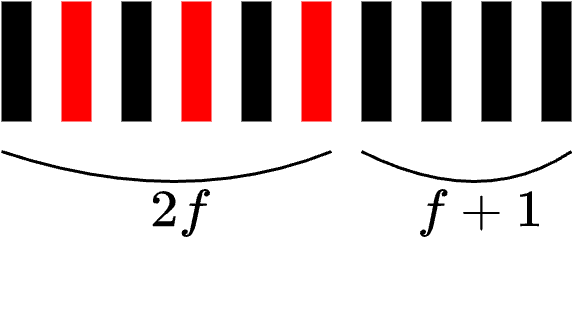
\includegraphics[scale=0.6]{lemma1.png}
	\caption{Example of round-robin leader allocation for $f = 1$. Red rectangles denote byzantine leaders.}
	\label{lemma1diagram}
\end{figure}

\begin{lemma} \label{viewslemma}
	There exists an infinite number of consecutive assignments of two honest leaders to views. That is, we can always find future consecutive views $v_1$ and $v_2$ with honest leaders.
\end{lemma}

\begin{proof}
	We use a round-robin system to allocate leaders to views. If we attempt to alternate honest and byzantine leaders, there will always be $f + 1$ consecutive honest leaders left over (figure \ref{lemma1diagram}). Hence there will always be at least 2 consecutive honest leaders (the lemma holds trivially for $f = 0$).
\end{proof}

\begin{lemma} \label{progressionlemma}
	An honest replica $x$ will eventually enter a view where it is leader.
\end{lemma}

\begin{proof}
	In the event that a byzantine node is leader and tries to prevent honest nodes from transitioning to a higher view, the honest nodes will eventually timeout and send a COMPLAIN message to the next leader (algorithm \ref{pacemaker}, line \ref{code_timeout}). This may repeat if the next leader is also byzantine. Eventually the COMPLAINs will be sent to an honest leader, that will send a NEXT{\large V}IEW message and transition all replicas into a new view (algorithm \ref{pacemaker}, line \ref{code_nextviewmsg}). Since $x$ will always progress to a higher view, it will eventually reach a view where it is the leader.
\end{proof}

\begin{theorem}[Synchronisation validity] \label{syncvalid}
	The pacemaker will only advance the view if at least one honest consensus machine\footnote{For this proof we consider the consensus machine (algorithm \ref{hotstuff}) and the pacemaker (algorithm \ref{pacemaker}), to be separate entities.} requests it to be advanced.
\end{theorem}

\begin{proof}
	This holds trivially for the calls to ON{\large N}EXT{\large S}YNC{\large V}IEW in algorithm \ref{hotstuff}, as the view is advanced on the request of the consensus machine.

	The only other way the view can be advanced, is on the receipt of a QC (algorithm \ref{pacemaker}, line \ref{code_gotqc}). For a QC to be formed a quorum of $n - f$ nodes must have complained or voted; at least one of these must have been an honest consensus machine that requested for the view to be advanced.
\end{proof}

%prove that it doesn't break safety
%maybe try to prove liveness
% https://decentralizedthoughts.github.io/2021-09-30-distributed-consensus-made-simple-for-real-this-time/
\section{Performance improvements} \label{performance}

\textit{In this section we highlight the key performance optimisations we implemented, and describe some of the debugging and experimentation that led to them. [this is a hard problem, reference chubby again. bugs are subtle.]}


% Batching \& limiting of batch sizes. deduplication in batching
% Send to all

% We give cases of deadlock conditions
% and performance issues / improvements found from debugging traces:
% 1. print statements (even when not in-between timing commands) can affect the time measured in another operation. Removed prints and printed all results at the end (use static collector function for logging that is passed around the program).
% 2. >= used lexicographic ordering, resulted in chains being verified due to first field being increasing until a specific command "20" where the value became lexicographically decreasing
% 3. Infinitely recursive start node not compatible nice with messaging system
% 4. Memory usage massively increased due to recursive node functions, replaced with an offset
% 5. Store a hash in each node and use it to compare nodes rather than checking their entire history
% 6. Discarding messages from future views results in some leaders not progressing
\subsection{Batching} \label{batching}
% mention send to all & send to one, 4x throughput
% reference latency graphs from final
One way to improve goodput (number of requests committed) is to `batch' requests, meaning a node may contain many commands instead of just one. This can dramatically increase goodput as now a single view can result in many commands being committed and executed instead of just one.

In order to implement this change in algorithm \ref{pacemaker} one simply has to modify the ON{\large N}EXT{\large S}YNC{\large V}IEW procedure. Instead of taking a single element from the queue of commands waiting to be proposed, the whole queue will be `batched' into a single proposal.

In theory this change should result in much higher goodput without any significant increase in latency. Analysis of timing data after implementing this feature revealed that latency had increased substantially. We now present some of the analysis and experimentation that was carried out to diagnose this issue. As mentioned in \ref{testing}, the nature of the project meant that debugging had to be carried out by manual inspection of the program trace and timing sections of the program. To overcome this I carried out tests in a scientific manner, constructing a hypothesis for why the program was slow based on crawling through logs, then attempting to test my hypothesis while controlling other variables, and finally implementing a solution.

\subsubsection{Probing effects}
% development of logging framework, some details of what is logged
I added timing and logging statements to key parts of the program, allowing me to better diagnose the source of the poor performance. Running a live test with print statements has the advantage that one can quickly see when progress is not being made, or when there are pauses, as the print statements stop. However, this benefit is outweighed by the sheer volume of logs and times being printed, it becomes difficult to manage when logs are in the millions of lines long.

Moreover, debugging by print statements had a bigger problem of inconsistencies between runs making it difficult to diagnose any problem. This was because the large volume of print statements being executed had a significant effect on the performance of the program. This is known as a \textit{probing effect}, the behaviour of a system is altered by the act of measuring it. I initially assumed that because the print statements were not in-between the timing statements they would not affect my measurements, but they are an expensive operation that can cause delays to happen in execution where one would not expect [cite???].

This problem was overcome through the development of a simple logging framework. Key parts of the program such as the state machine advancing, actions being carried out, messages being sent, are all timed and added to lists. Critically, this list is stored and not printed out until the node is killed, so the printing cannot interfere with execution. Relevant statistics such as mean, standard deviation, and total time for each interval measured are outputted, providing crucial insight into the performance of the program.

\textbf{Design principle: } Minimise probing effects by carrying out the minimum possible amount of work in critical areas of the program, storing data, and moving work (such as outputting statistics) to less critical areas of the program.

\subsubsection{Architectural experimentation}
% https://outlook.office.com/mail/id/AAQkADc5ODY2YTdlLTQ3NGMtNDVmOS05ZDAxLWNhYzkwMjU2MThhZAAQADc%2B0AASzwxBgZSNOjdNZ%2Bw%3D
% development of architecture in overview
% tried moving to non event-driven model
% thought resource contention was issue, in fact it was async get function
Initial analysis of timing data showed a large amount of time was spent by requests queuing on the node before they are delivered to the state machine. At this time the architecture presented in section \ref{overview} had not been fully developed, specifically, there was only one stream that contained both internal messages and client requests.

\textbf{Hypothesis: } Internal messages are being starved by client requests. At large throughputs the stream quickly becomes filled with client requests, which may prevent internal messages being handled. Internal messages represent a backlog of work that is not yet finished, so this should be handled before accepting more requests.

\textbf{Design principle: } The system should prioritise clearing its backlog of work before accepting new work.

\textbf{Potential solution: } Split the stream into two separate streams for messages and requests, and always pick from the message stream over the request stream until the message stream is empty.

Implementing the potential solution did not lead to a significant improvement in performance, so this was not the issue. However, this architectural model was retained as it is theoretically better and may lead to observable improvements later.

Another potential cause of the issue was that internal messages are starving client requests, rather than the other way around. The modified implementation of the pacemaker (\ref{spec}) immediately begins a new view as soon as the previous one is finished, which causes a large amount of internal messages.

\textbf{Hypothesis: } Because the state machine is constantly advancing at the fastest possible rate, the volume of internal messages may prevent new requests from being handled.

\textbf{Experimentation: } One approach is to `balance' the starvation by mostly prioritising internal messages, but every \textit{x} iterations picking a request instead of an internal message. Varying \textit{x} led to significant changes in performance, but no value for \textit{x} led to a good level of performance. This approach did not appear workable, as the nature of starvation seemed to be a complicated, with messages starving requests, and the other way around.

\textbf{Potential solution: } Instead of starting the next view whenever possible, deliver the \textit{BEAT} and \textit{ON{\large N}EXT{\large S}YNC{\large V}IEW} interrupts at a steady rate.

This potential solution was implemented; it involved checking a timer on every iteration of the main loop to see if some $\Delta$ had elapsed and it was time to deliver the next interrupt, as well as significant modifications to be made to the consensus state machine. Implementing this feature actually led to a significant performance hit, so the changes were discarded. However, experimenting with this feature showed an interesting phenomenon; the main loop, which is infinitely recursive, was running at a much slower rate than one would expect. Further timing statements revealed that the command which removed an element from the stream would sometimes take a very long time (on the order of seconds). Reading more into the Lwt documentation led to the following idea:

\textbf{Potential solution: } Use a different method to take elements from the queue that is synchronous. This should stop the main loop blocking waiting for the queue to fill up.

This change improved performance by reducing the amount of time spent waiting in the main loop.

\subsubsection{Send-to-all and filtering} \label{sendtoall}
% send to all weird graph: https://outlook.office.com/mail/id/AAQkADc5ODY2YTdlLTQ3NGMtNDVmOS05ZDAxLWNhYzkwMjU2MThhZAAQAM2hZuzkpUNIuGt2QHNZQvc%3D
% exponential growth with end to all https://imgur.com/a/wDlhbn9 28/03 pseudocode
% theory: nodes reproposing same values
% first solution: deduplicate before commiting, use set instead of queue
% second solution: deduplicate based on *seen* commands
% could mention bug of reawaking the same promise in the hash table - this brought to my attention the deduplication issue!
Further problems were uncovered by the implementation of send-to-all in the load generator (section \ref{benchcode}). Without this feature a client would randomly chose a node to send their request to, and the command would not be proposed until the round-robin system reached that node to become the leader. Send-to-all can reduce latency by instead broadcasting a request to all nodes, meaning that the next leader can propose the command without having to wait for the round-robin system to reach them.

Instead of reducing latency as expected the implementation of this feature actually led to dramatically increased latency, and some requests not being fulfilled at all within the time that the experiment ran. Heatmaps that show the distribution of latencies over the course of an experiment showed that latency increased exponentially over the course of the test.

\textbf{Hypothesis: } Send-to-all overloads the system by increasing the number of requests by a factor of \textit{n}, where \textit{n} is the number of nodes.

\textbf{Experimentation: } If our hypothesis is true, then we should see similar behaviour in a send-to-one system run at \textit{n} times the throughput. This is indeed the case; running a send-to-one system with such high throughput led to exponential growth in latencies.

\textbf{Further evidence: } Implementing this feature resulted in Lwt errors being thrown. As described in \ref{overview}, in order to respond to client requests, the node maintains a hash table of promises that can be awakened when the consensus state machine has successfully committed and can respond to the client. The Lwt error was caused by promises stored in the hash table being awoken multiple times, which causes an error. This provides further evidence that the same commands are being committed and responded to multiple times, which is wasted work.

\textbf{Potential solution: } Filter commands in the system to minimise the number of commands that are proposed by multiple nodes.

\textbf{Design principle: } Attempt to minimise the amount of redundant work that the system carries out by screening incoming work to check that it actually needs to be done.

One way to implement this is to maintain a set of commands that have been committed, and before proposing or committing a node, calculating the set difference with the \textit{commited} set to filter out redundant commands. Instead of nodes containing a list of commands, as in our naive implementation of batching, we now use a set to enable efficient computation of the difference.

\begin{algorithm}[h!]
	\caption{Filtering implementation \#1}
	\begin{algorithmic}[1]
	\Procedure{ON{\large C}OMMIT}{\textit{b}}
		\If{$\textit{b\textsubscript{exec}.height} < \textit{b.height}$}
			\State $\textit{toCommit} \gets \textit{b.cmds} \setminus \textit{commited} $
			\State $\textit{commited} \gets \textit{commited} \cup \textit{toCommit}$
			\State $\text{ON{\large C}OMMIT}(\textit{b.parent})$
			\State $\text{EXECUTE}(\textit{toCommit})$
		\EndIf
	\EndProcedure
	\Procedure{ON{\large N}EXT{\large S}YNC{\large V}IEW}{$\textit{view}$}
		\State $ \textit{curView} \gets \textit{view}$
		\State $ \text{ON{\large B}EAT}(\textit{cmds} \setminus \textit{commited})$
		\State $ \textit{cmds} = \{\}$
		\State \textcolor{gray}{//\ \dots}
	\EndProcedure
	\Procedure{ON{\large R}ECIEVE{\large C}LIENT{\large R}EQUEST}{\text{REQ}(\textit{cmd})}
		\State $ \textit{cmds} \gets \textit{cmds} \cup \{\textit{cmd}\} $
	\EndProcedure
	\end{algorithmic}
\end{algorithm}

This implementation did not lead to the desired reduction in latency, the system still exhibited the exponential growth previously observed. The lack of change in observable behaviour implied that the filtering of requests was not happening successfully.

\textbf{Hypothesis: } A command (\textit{x}) is committed four views after it is proposed. In these four views our deduplication is ineffective in screening \textit{x} from being proposed again. Notably another node will not try to commit \textit{x} for a second time, but the data indicates that being proposed multiple times is a more important factor affecting performance. 

\textbf{Experimentation: } Count the elements that are filtered out from being proposed by measuring the value $|\textit{cmds}| - |\textit{toPropose}|$. This value was small, which supports the hypothesis that filtering was largely ineffective.

\textbf{Potential solution: } Screen incoming commands more aggressively by instead maintaining a set of any commands that have been \textit{seen}. Only filter out commands when they are being proposed rather than when they are being committed, as there is no evidence that screening at commit time gives any tangible benefit.

\begin{algorithm}[h!]
	\caption{Filtering implementation \#2} \label{dedup2}
	\begin{algorithmic}[1]
	\Procedure{ON{\large R}ECEIVE{\large P}ROPOSAL}{$\text{MSG}\textsubscript{\textit{v}}(\text{GENERIC}, \textit{b\textsubscript{new}}, \textit{qc})$}
		\If {$ v = \text{GET{\large L}EADER}(\textit{m.view}) \land \textit{m.view} = curView$}
			\State $ \textit{seen} \gets \textit{seen} \cup \textit{b\textsubscript{new}.cmds}$
			\State \textcolor{gray}{//\ \dots}
		\EndIf
	\EndProcedure
	\Procedure{ON{\large N}EXT{\large S}YNC{\large V}IEW}{$\textit{view}$}
		\State $ \textit{curView} \gets \textit{view}$
		\State $ \text{ON{\large B}EAT}(\textit{cmds} \setminus \textit{seen})$
		\State $ \textit{cmds} = \textit{seen} = \{\}$ \label{smalloptimisation}
		\State \textcolor{gray}{//\ \dots}
	\EndProcedure
	\Procedure{ON{\large R}ECIEVE{\large C}LIENT{\large R}EQUEST}{\text{REQ}(\textit{cmd})}
		\State $ \textit{cmds} \gets \textit{cmds} \cup \{\textit{cmd}\} $
	\EndProcedure
	\end{algorithmic}
\end{algorithm}

Note the small optimisation on line \ref{smalloptimisation}, the \textit{seen} can safely be emptied as the commands have already been filtered; this reduces the amount of computation required to calculate the set difference next time. The second implementation was much more effective at screening requests and resulted in a significant reduction in latency. The difference is demonstrated in an ablation study (section \ref{ablation}) The effectiveness of this change led to further insight into what the bottlenecks for performance were.

\subsubsection{Batch sizes} \label{batchsizes}
% insight: track batch sizes
% experimented with limiting batch size
% tie into benchmarking of cap'n proto
The effectiveness of filtering out commands to make proposals smaller implies that the size of a proposal has a significant impact on the performance of the program. Furthermore, analysis of the time data for sending messages showed that there was a high variance in time taken, with some messages taking on the order of milliseconds [verify ***] to be sent.

\textbf{Hypothesis: } Large batches of commands cause messages to become larger, which causes them to be sent slowly due to limitations in the RPC framework.

\textbf{Potential mitigation: } Limit the size of batches to prevent messages becoming too large.

Implementing this feature required minimal changes to algorithm \ref{dedup2}, one simply has to take a subset of \textit{cmds} to propose instead of the whole set. This feature gave a significant performance improvement, and largely eliminated the exponential growth in latency that had been seen previously. There is a trade-off between sending larger batches (more commands are committed, but messages take longer to send) and sending smaller batches (less commands are committed, but messages are sent faster). This trade-off is explored more in our analysis of the system with different batch sizes [refer to evaluation***]. Fundamentally, there are limitations in the RPC framework that give an upper bound on the performance we can hope to achieve, these limitations are evident in our benchmarking of the Cap'n Proto framework (\ref{capnpbenchmark}).
\subsection{Encoding of nodes}
% https://outlook.office.com/mail/id/AAQkADc5ODY2YTdlLTQ3NGMtNDVmOS05ZDAxLWNhYzkwMjU2MThhZAAQALSHx8XQgvxMrG5AvVEd9as%3D
% 19/01 onwards
% first issue: infintely recursive node structure
% solution: hardcoding final node at either end so it is not sent
% second issue: growing memory usage - revealed by profiling
% solution: use offset to node, and reconstruct node at either end. introduce `justify' type
% third issue: memory usage comparing nodes
% solution: include node hashes
% fourth issue: size of sending all nodes
% solution: TODO implement TCP
\textit{This section concerns the difficulties of encoding nodes in the Cap'n Proto schema, and designing a suitable type to represent them. As mentioned in \ref{overview}, Cap'n Proto requires a schema to define the format of RPCs that can be sent, and one must convert between consensus state machine internal types and Cap'n Proto types in order to send messages.}

\subsubsection{Recursive types}
The unchained HotStuff algorithm has a genesis node \textit{b\textsubscript{0}} that starts the chain of nodes. Each node contains the fields \textit{parent}, \textit{cmd}, \textit{justify}, and \textit{height}, with the \textit{justify} field containing a quorum certificate with a `pointer' to another node in the chain (section \ref{chaining}). The genesis node \textit{b\textsubscript{0}} contains a hardcoded link to itself, so $ b_0.\textit{justify}.\textit{node} = b_0$.

This recursion poses a problem when carrying out the conversion between Cap'n Proto types and OCaml types. It is perfectly possible to define a recursive type in OCaml, so one can represent \textit{b\textsubscript{0}} inside the consensus state machine. However, the naive implementation of a function to convert this node into a Cap'n Proto type will not terminate, as it will infinitely recurse into the field $ b_0.\textit{justify}.\textit{node} $. A simple solution to this problem is to add a flag to the Cap'n Proto schema \textit{is\_b\textsubscript{0}}; when this flag is enabled then the node is assumed to be equal to \textit{b\textsubscript{0}}. This prevents \textit{b\textsubscript{0}} from ever having to be converted into a Cap'n Proto type or being sent over the network, it can instead be reconstructed as a recursive type in the consensus state machine of the receiver.

\subsubsection{Node offsets}
During live testing, memory usage increased rapidly, the nodes quickly exceeded the amount of memory the system had, and their processes were killed by the OS. Profiling with Memtrace (section \ref{testing}) showed that the functions for converting between Cap'n Proto types and internal consensus types was responsible for the rapidly increasing memory usage.

This problem arose from the internal types that were designed to represent nodes. As well as the \textit{node} type, there was a \textit{qc} type that was used as the type of the \textit{node.justify} field since it is a quorum certificate. By defining types in this way the `pointers' in \textit{node.justify.node} were not actually pointers, they contained a significant part of the chain. In this way the chain contained many redundant copies of parts of it, resulting in a very bloated \textit{node} object that was very expensive to convert.

A solution to this problem is to store an offset to a node inside the \textit{justify} field rather than the node itself - making it more like a real pointer. This offset represents how many \textit{parent} links away the node is, and so can be used to reconstruct all of the original information. To implement this another type \textit{node\_justify} was added, that is identical to \textit{qc}, but with the field \textit{node} replaced with \textit{node\_offset}. One must then convert between the \textit{node\_justify} and \textit{qc} types to reconstruct the original data and follow the \textit{node.justify.node} link.

\subsubsection{Node comparison}
Memtrace profiling also showed that the equality function for nodes was memory intensive. The solution to this was including a \textit{digest} field in the node that is a hash over all of the other fields. Notably we can compute this hash over the \textit{digest} field of the parent node rather than recursing through the whole chain. This means that we can also compare two nodes by comparing their digests without having to recurse through each chain; the digests being equal cryptographically guarantees that the whole chains are equal.

\subsubsection{Node truncation} \label{truncation}
Our current approach sends the entire node inside internal messages, which becomes expensive as the chain grows. As highlighted in section \ref{batchsizes}, the size of messages being sent is a bottleneck in the system, making this particularly expensive.

In order to overcome this problem, one can truncate the node before sending it, cutting off the node's parent link at some chosen depth. The entire node can then be reconstructed at the receiver, the received node can be `spliced' back together with \textit{b\textsubscript{exec}}, which contains the node up to the point that has been executed. However, we must ensure not to truncate the log too much, so that there is a gap between what we send and \textit{b\textsubscript{exec}} at the receiver, leading to commands being missed out and not executed. This is a problem in the event that some node becomes isolated from the rest; it must be able to catch up to the others once the network partition is healed.

To overcome this problem we use a TCP-style approach. We include a field containing the height of the \textit{b\textsubscript{exec}} node to the \textit{PROPOSE}, \textit{NEW{\large V}IEW}, and \textit{COMPLAIN} messages. Each node maintains a list of the \textit{b\textsubscript{exec}} height of every other node. When making a proposal, the leader takes the minimum height from this list, and truncates the node up to that depth. This ensures that every node that receives the proposal has enough information to reconstruct the entire log.

There are some cases when the leader does not receive the latest \textit{b\textsubscript{exec}} of every other node before it makes a proposal. This means that the leader will not truncate the node as much as it could have. We optimised this by having a node send the entire list of all stored \textit{b\textsubscript{exec}} heights rather than just its own, allowing the heights to propagate around the system more quickly.

% \subsection{Connections}
% talk about capabilities?
% when to set up connections? use promises
% https://outlook.office.com/mail/id/AAQkADc5ODY2YTdlLTQ3NGMtNDVmOS05ZDAxLWNhYzkwMjU2MThhZAAQAEXEcHtcUNFFo%2FRcUtQcSmc%3D

% \section{Verifiable anonymous identities}
% https://www.usenix.org/system/files/nsdi22-paper-shamis.pdf
% section 5

\section{Implementing for evaluation} \label{benchcode}
% Benchmarking code
% discuss open loop vs closed loop clients
% avoid coordinated ommision by using open loop clients
% section 3: https://dl.acm.org/doi/pdf/10.1145/3447851.3458739

\textit{In this section we describe the infrastructure that will be used to evaluate our system in chapter \ref{evaluation}, including the scripting developed to automate running experiments.}

\subsection{Load generator} \label{loadgenerator}

\begin{figure}[h]
\centering
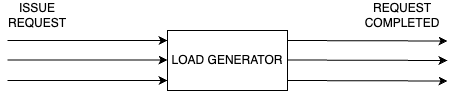
\includegraphics[scale=0.6]{openloop.png}
\caption{Open-loop load generator.}
\label{openloop}
\end{figure}

\begin{figure}[h]
\centering
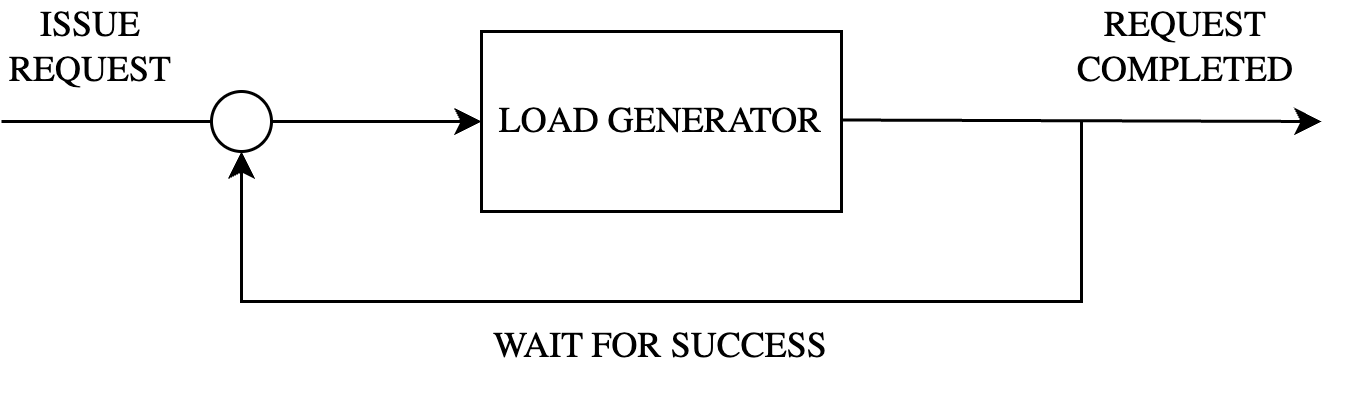
\includegraphics[scale=0.6]{closedloop.png}
\caption{Closed-loop load generator.}
\label{closedloop}
\end{figure}

The load generator is responsible for sending client requests to the nodes of the system. One is able to vary the throughput that the load generator drives the system at, and the duration that it runs for before it sends a \textit{kill} messages to the nodes, ending the test. It is also responsible for timing and calculating statistics.

\textbf{Throughput: } The number of requests sent by the load generator each second.

\textbf{Goodput: } The number of requests that are responded to each second. This is calculated by number of responses divided by the time difference between the first response and the end of the test.

\textbf{Latency: } The amount of time it takes between sending a request and receiving a response. The load generator reports both mean and standard deviation of latencies.

The load generator is open-loop (figure \ref{openloop}), which means that it dispatches a request every $\delta$ seconds for the duration of the experiment, where $\delta = \frac{1}{\textit{throughput}}$. This is in contrast to a closed-loop generator (figure \ref{closedloop}), which must wait until it receives a response in order to send the next request. An open-loop load generator is more useful for our experiments as it allows us to overload the system and test its limits, whereas a closed-loop load generator `waits' for the system, so cannot overload it.

The load generator uses Lwt to asynchronously dispatch requests, and stores a promise that will be fulfilled with their response. In the case of send-to-all (\ref{sendtoall}) the promises waiting on a response from each node are combined using \textit{Lwt.pick}, meaning that the first node to respond will fulfil the promise and the rest will be ignored. Before beginning the experiment the load-generator sends `dummy' requests to each node until all of them have sent a response; this ensures that all nodes are properly up and running before we start the experiment, eliminating start-up effects.

\subsection{Experiment scripts} \label{experimentscripts}
Python scripts are used to automate the running of experiments. These scripts start the nodes and the load generator, wait for the experiment to run, kill the processes, run a script to plot graphs, then start the next experiment.

Different experiments may vary input variables such as throughput, batch size, and number of nodes. The script takes all possible permutations of the input variables, duplicates them (so that each experiment is run multiple times to get better results), and runs them in a random order. By running experiments in a random order external factors that affect performance are somewhat mitigated. For example if the experiments were not run in a random order, the system may happen to experience interference when running experiments on 8 nodes, giving distorted results for this set of experiments. If instead the experiments were run randomly, the interference would affect some random group of experiments, and it would be more apparent that these results were anomalous. [could be more concise]

\section{Repository Overview} \label{repo}

\begin{small}
\begin{forest}
	for tree={font=\sffamily, grow'=0,
	folder indent=0.9em, folder icons,
	edge=densely dotted}
	[src
		[\ consensus,
			[consensus\_chained\_impl.ml, is file]
			[consensus\_impl.ml, is file]
			[consensus.ml, is file]
			[consensus.mli, is file]
			[crypto.ml, is file]
			[types.ml, is file]
			[types.mli, is file]
			[util.ml, is file]
		]
		[\ experiments
			[\ data]
			[\ graphs]
			[plot.py, is file]
			[plotDummy.py, is file]
		]
		[hs\_api.capnp, is file]
		[api\_wrapper.ml, is file]
		[api\_wrapper.mli, is file]
		[dummy.ml, is file]
		[hs.ml, is file]
		[live\_test.ml, is file]
		[main.ml, is file]
		[net.ml, is file]
		[types.ml, is file]
		[util.ml, is file]
		[runDummyExperiments.py, is file]
		[runExperiments.py, is file]
		[README.md, is file]
	]
\end{forest}
\end{small}

The \textit{src} directory contains the main server loop and the code for interacting with Cap'n Proto to send messages. It also contains code for the load generator, and Python scripts to run experiments and benchmarks. Inside the \textit{consensus} folder is the implementation of the consensus library based on the pseudocode presented in \ref{spec}. N.B. this folder also contains testing files that are omitted for conciseness. The \textit{experiments} folder is where the data from running experiments is outputted to, and it contains scripts for plotting graphs.

In order to run an experiment, first follow the instructions in \textit{README.md} to set up your environment. You can then run experiments by executing \textit{python3 runExperiments.py}, and modify this script to vary the input parameters such as throughput and experiment time. These scripts will run on Linux and MacOS, but will have to be modified to work on Windows.